%%%%%%%%%%%%%%%%%%%%%%%%%%%%%%%%%%%%%%%%%%%%%%%%%%%%%%%%%%%%%%%%%%%%%%
%
% Institut für Rechnergestuetzte Automation
% Forschungsgruppe Industrial Software
% Arbeitsgruppe ESSE
% http://security.inso.tuwien.ac.at/
% lva.security@inso.tuwien.ac.at
% 
%%%%%%%%%%%%%%%%%%%%%%%%%%%%%%%%%%%%%%%%%%%%%%%%%%%%%%%%%%%%%%%%%%%%%%

\documentclass[12pt,a4paper,titlepage,oneside]{scrartcl}
\usepackage{esseProtocol}

%%%%%%%%%%%%%%%%%%%%%%%%%%%%%%%%%%%%%%%%%%%%%%%%%%%%%%%%%%%%%%%%%%%%%%
%
% FOR STUDENTS
%
%%%%%%%%%%%%%%%%%%%%%%%%%%%%%%%%%%%%%%%%%%%%%%%%%%%%%%%%%%%%%%%%%%%%%%

% Group number or "0" for Lab0
\newcommand{\gruppe}{AG\_ue\_11}
% Date
\newcommand{\datum}{05.06.2012}
% valid values: "Lab0", "Lab1" (be sure to use Uppercase for first character)
\newcommand{\lab}{Lab1}

% name of course, for example: "IT Security in Large IT Infrastructures", "Security for Systems Engineering", "Introduction to Security"
\newcommand{\lvaname}{IT Security in Large IT Infrastructures}
% number of course, for example: "183.633", "183.637", "183.594"
\newcommand{\lvanr}{183.633}
% year and term, for example: "SS 2012", "WS 2012", "SS 2013", etc.
\newcommand{\semester}{SS 2012}

% Student data in Lab0 or first student of group in Lab1
\newcommand{\studentAName}{Stephan Klein}
\newcommand{\studentAMatrnr}{0825294}
\newcommand{\studentAEmail}{e0825294@student.tuwien.ac.at}

% second student of group in Lab1, for Lab0 you may leave it unchanged
\newcommand{\studentBName}{Paul Apo Gültekin}
\newcommand{\studentBMatrnr}{0926967}
\newcommand{\studentBEmail}{e0926967@student.tuwien.ac.at}

% second student of group in Lab1, for Lab0 you may leave it unchanged
\newcommand{\studentCName}{Andreas Ofner}
\newcommand{\studentCMatrnr}{0247950}
\newcommand{\studentCEmail}{e0247950@student.tuwien.ac.at}

% second student of group in Lab1, for Lab0 you may leave it unchanged
\newcommand{\studentDName}{Jürgen Unger}
\newcommand{\studentDMatrnr}{0827133}
\newcommand{\studentDEmail}{e0827133@student.tuwien.ac.at}

%%%%%%%%%%%%%%%%%%%%%%%%%%%%%%%%%%%%%%%%%%%%%%%%%%%%%%%%%%%%%%%%%%%%%%
%
% DO NOT CHANGE THE FOLLOWING PART
%
%%%%%%%%%%%%%%%%%%%%%%%%%%%%%%%%%%%%%%%%%%%%%%%%%%%%%%%%%%%%%%%%%%%%%%

\newcommand{\dokumenttyp}{Abgabedokument \lab}

\begin{document}

\maketitle
\setcounter{section}{0}
\setcounter{tocdepth}{2}
\tableofcontents

%%%%%%%%%%%%%%%%%%%%%%%%%%%%%%%%%%%%%%%%%%%%%%%%%%%%%%%%%%%%%%%%%%%%%%
%
% CONTENT OF DOCUMENT STARTS HERE
%
%%%%%%%%%%%%%%%%%%%%%%%%%%%%%%%%%%%%%%%%%%%%%%%%%%%%%%%%%%%%%%%%%%%%%%

\section{Festlegung der Sicherheitsziele}
\subsection{Confidentiality}
Es soll vermieden werden, dass Informationen unauthorisiert aus dem System
ausgelesen werden können. In Bezug auf die einzelnen Module bedeutet das, dass
entsprechende Authentifizierungsmöglichkeiten geschaffen werden müssen, die auch
sicher implementiert werden.

\subsubsection{Bedrohungen}
\begin{itemize}
	\item Kompromittierung der Datenbank
	\item Kompromittierung des Betriebssystems
	\item Mitschneiden von unverschlüsseltem Netzwerktraffic
	\item Social Engineering
\end{itemize}

\subsection{Integrity}
Alles, was die gespeicherten Informationen unsicher oder unzuverlässig machen
kann, soll vermieden werden. Das bedeutet die konsequente Validierung aller
Eingabedaten sowohl von externen Quellen als auch im Datenaustausch zwischen den
einzelnen Modulen im System. Dadurch soll eine entsprechende Isolation der einzelnen
Komponenten erreicht werden, sodass ein kompromittiertes Modul nicht gleich das
Gesamtsystem in Gefahr bringt.

\subsubsection{Bedrohungen}
\begin{itemize}
	\item Kompromittierung der Datenbank
	\item Kompromittierung des Betriebssystems
	\item Manipulation von unverschlüsseltem Netzwerktraffic (Man in the Middle)
	\item Fehlende oder fehlerhafte Validierung der Eingabedaten
\end{itemize}


\subsection{Authentication}
Die unauthorisierte Veränderung von gespeicherter Information soll verhindert
werden. Damit werden entsprechende Authentifizierungsmöglichkeiten noch einmal
wichtiger.

\subsubsection{Bedrohungen}
\begin{itemize}
	\item Kompromittierung der Datenbank
	\item Kompromittierung des Betriebssystems
	\item Replay-Attacken auf die Authentifizierung
	\item Social Engineering
\end{itemize}

\subsection{Non-Repudiation}
Es soll möglich sein, den Sender wie auch den Empfänger von Informationen eindeutig
zu identifizieren. Durch eine Public Key Infrastructure (PKI) kann dieses Ziel
erreicht werden. Besonders bei der Verwaltung von Kredikartendaten und der
Durchführung von geschäftlichen Transaktionen ist es sowohl für den Betreiber
als auch für den Kunden von großem Interesse, dass nach Abschluss eines Geschäftes
keine Seite mehr behaupten kann, dass die Transaktion nicht stattgefunden hat.

\subsubsection{Bedrohungen}
\begin{itemize}
	\item Identitätsdiebstahl
	\item Replay-Attacken auf Transaktionen
	\item Social Engineering
\end{itemize}

\subsection{Access Control}
Es muss möglich sein, den Zugriff auf die einzelnen Komponenten und das Gesamtsystem
zu limitieren und zu kontrollieren. Durch die Vergabe und das Signieren von
Zertifikaten ist es möglich, je nach Zertifikat andere Funktionalitäten auf den
einzelnen Modulschnittstellen freizugeben. Soll ein Modul nicht mit einem anderen
kommunizieren dürfen (weil es etwa nicht notwendig ist), kann der Zugriff so
auch direkt blockiert werden.

\subsubsection{Bedrohungen}
\begin{itemize}
	\item Kompromittierung der Datenbank
	\item Kompromittierung des Betriebssystems
	\item Fehlerhafte Verteilung bzw. Verlust von Zugangsdaten
	\item Social Engineering
\end{itemize}

\subsection{Availiability}
Es soll verhindert werden, dass die im System gespeicherten Informationen
unauthorisiert vorenthalten werden. Das bedeutet, dass das System seinen Dienst
tun soll und seine Funktionalität diejenigen zur Verfügung stellen soll, die dazu
auch befugt sind.

\subsubsection{Bedrohungen}
\begin{itemize}
	\item (Distributed) Denial of Service
\end{itemize}

\section{Beschreibung und Definition der Schnittstellen}

\subsection{Allgemeines zur Kommunikation zwischen den Services}
Alle Services mit Ausnahme des Kartenterminals und des Benachrichtungsdienstes
kommunizieren über verschlüsselte HTTP-Verbindungen, die via 2-Way SSL Handshakes
hergestellt wird. Dadurch wird bei jeder Interaktion die Identität der beteiligten
Komponenten sichergestellt.

\subsubsection{Servicekommunikation und Nachrichtenformat}
Die einzelnen Serviceaufrufe passieren über REST-Services. Daten werden
ausschließlich in JSON übertragen. Die Antworten der Module sind standardisiert
und können entweder Einzelwerte, Listen oder assoziative Arrays (Dictionaries)
als Antwort liefern:

\begin{lstlisting}
{ "result": 231 }
{ "result": [1, 2, 3] }
{ "result": { "foo": "bar", "answer": 42 } }
{ "result": [ { "foo": "bar" }, { "beep": "boop" }] }
\end{lstlisting}

Die HTTP-Response-Codes sind im Erfolgsfall je nach verwendetem HTTP-Verb
unterschiedlich. Bei \texttt{GET}, \texttt{DELETE} wird \texttt{200 OK}, bei
\texttt{POST} wird \texttt{201 Created} zurückgegeben.

Im Fehlerfall wird \texttt{400 Bad Request} zurückgegeben.
Als Body wird eine entsprechende Fehlermeldung übertragen.

\begin{lstlisting}
{ "error": { "message": "A detailed description of the error." } }
\end{lstlisting}

\subsection{Kundenmanagement}
\subsubsection{Anforderungen}
Das Kundenmanagement wird verwendet, um Kundendaten zu verwalten.
Zu den gespeicherten Daten zählen:

\begin{itemize}
	\item [*] Kundennummer
	\item [*] Vorname und Nachname
	\item [*] Loginname
	\item [*] Passwort
	\item [**] Geburtsdatum
	\item [**] Adressdaten (PLZ, Straße, Ort, Staat)
	\item [**] Kontaktdaten (Telefonnummer, Emailadresse, …)
	\item [**] Bankverbindung (IBAN, BIC)
\end{itemize}

Die gespeicherten Daten lassen sich in sensible (*) und sehr sensible Daten (**) klassifizieren.
Sensible Daten können im Klartext gespeichert werden, sind jedoch gegen unauthorisierten
Zugriff auf Modul- und Datenbankebene zu sichern. Sehr sensible Daten dürfen nur
in verschlüsselter Form in einer separaten Tabelle abgespeichert werden. Diese
Tabelle ist auf Datenbankebene gegen unbefugten Zugriff besonders zu schützen.

Um den sicheren Umgang mit diesem Modul zu gewährleisten muss zwischen den Schnittstellen
zur Kartenverwaltung und zu den (Self-)Managementsystemen unterschieden werden.

Die JSON-Serialisierung eines Kundenobjektes sieht folgendermaßen aus:
\begin{lstlisting}
{
  "result":{
    "id":"029322312",
    "name":"Mustermann",
    "firstname":"Max",
    "login":"mmustermann",
    "password":"DEADBEEF",
    "birthday":"1980-01-01",
    "adresses":[
      {
        "type":"postal",
        "street":"Musterweg 12",
        "zip":1010,
        "city":"Vienna",
        "country":"Austria"
      },
      {
        "type":"email",
        "email":"max@mustermann.at"
      }
    ],
    "payment":[
      {
        "iban":"1234567890",
        "bic":"AT12346"
      }
    ]
  }
}
\end{lstlisting}

\subsubsection{Schnittstelle: Kartenverwaltung}
Die Kartenverwaltung hat nur Lesezugriff auf Kundenobjekte.
\begin{description}
\item[GET /customer]
	Ruft ein Kunden-Objekt ab. Parameter: \texttt{id} (Kundennummer)
\end{description}

\subsubsection{Schnittstelle: Administrationsservices}

Für die verschiedenen Administrationsservices soll ein entsprechendes
Rechteverwaltungssystem implementiert werden. Je nach Berechtigung werden die
retounierten bzw. empfangenen JSON-Objekte gefiltert.

Benutzer des Mitarbeiterbackends dürfen sämtliche Datenkategorien bearbeiten.
Kunden, die sich über die Self-Management-Webseite einloggen (mit SSL
gesicherte Verbindung mit Passwort-Authentifizierung) können keine sehr
sensiblen Daten verändern.

Das Mitarbeiterbackend muss so wie die anderen Module über eine mittels 2-Way-SSL
gesicherte Verbindung mit der Kundenverwaltung kommunizieren.

\begin{description}
\item[POST /customer]
	Legt einen neuen Kunden an.

\item[DELETE /customer]
	Löscht einen Kunden. Parameter: \texttt{id} (Kundennummer)

\item[PUT /customer]
	Aktualisiert einen Kunden.

\item[GET /customer]
	Ruft ein Kunden-Objekt ab. Parameter: \texttt{id} (Kundennummer)

\end{description}


\subsection{Kartenverwaltung}
\subsubsection{Anforderungen}
Die Kartenverwaltung soll eine sichere und nachvollziehbare Verwaltung der sich im Umlauf befindlichen Karten gewährleisten. Weiters bietet das Service die Möglichkeit, Karten auf ihre Gültigkeit und auf ihr Limit zu testen.

Eine Karte ist durch das Tupel (Kartennummer, Gültigkeitsdatum) eindeutig identifiziert. Um eine Gültigkeits- oder Limitabfrage durchzuführen ist es notwendig, alle Elemente dieses Tupels zu kennen. Folgende Daten werden für jede Kreditkarte gespeichert:

\begin{itemize}
    \item validity (Gültigkeitsdatum)
    \item limit (Dezimalwert, der das Limit beschreibt)
    \item cardno (String, der via Regular Expression auf DB-Ebene validiert wird)
    \item customer (Referenz auf einen Kunden in der Kundenverwaltung)
    \item signature (in Base64)
\end{itemize}

Die JSON-Serialisierung eines Kartenobjektes sieht folgendermaßen aus:
\begin{lstlisting}
{
  "cardno":"9876543210",
  "validity":"09/14",
  "limit":2000.0,
  "customer":31,
  "signature":"BA423GHA...8=="
}
\end{lstlisting}

\subsubsection{Schnittstelle: Transaktionsverwaltung}
Die Transaktionsverwaltung hat nur lesenden Zugriff auf das Modul.
\begin{description}
	\item[GET /card/isValid]
		Überprüft, ob eine Karte gültig ist. Dabei werden die gespeicherten Daten auf Gültigkeit geprüft, um Manipulationen direkt an der Datenbank auszuschließen. Eine Karte ist genau dann gültig, wenn in der Datenbank genau ein Treffer für die übergebenen Parameter vorhanden ist, das Gültigkeitsdatum in der Zukunft liegt, die Karte einem Kunden zugeordnet ist und die digitale Signatur korrekt ist. Parameter: \texttt{cardno} (Kartennummer), \texttt{validity} (Gültigkeitsdatum)
		
		\begin{lstlisting}
		{ "result": true }
		\end{lstlisting}
		
	\item[GET /card/limit]
		Ruft das Limit für eine Karte ab. Dabei werden die gespeicherten Daten auf Gültigkeit geprüft, um Manipulationen direkt an der Datenbank auszuschließen. Parameter: \texttt{cardno} (Kartennummer), \texttt{validity} (Gültigkeitsdatum)
		
		\begin{lstlisting}
		{ "result": true }
		\end{lstlisting}
		
\end{description}

\subsubsection{Schnittstelle: Kundenverwaltung}
Diese Schnittstelle erbt sämtliche Funktionalität der Transaktionsverwaltung-Schnittstelle
und stellt darüber hinaus folgende Operationen zur Verfügung:

\begin{description}
	\item[POST /card]
		Erstellt eine neue Karte. Beim Anlegen prüft das Modul, ob der Kunde existiert, ob das Gültigkeitsdatum in der Zukunft liegt und ob die Signatur gültig ist. Die Signatur wird vom Kundenmanagement generiert und ist spezifisch für den Benutzer, der die Kundenverwaltung verwendet und die Anfrage stellt.

	\item[DELETE /card]
		Löscht die Karte mit der gegebenen Kartennummer. Parameter: \texttt{cardno} (Kartennummer), \texttt{validity} (Gültigkeitsdatum)
		
		\begin{lstlisting}
		{ "result": true }
		\end{lstlisting}

\end{description}

\subsection{Transaktionsverwaltung}
\subsubsection{Anforderungen}

Die Transaktionsverwaltung wird verwendet um eingehende Transaktionen abzuwickeln
und nachvollziehbar und rückverfolgbar zu dokumentieren.

Eine Transaktion besteht aus folgenden Daten:
\begin{itemize}
	\item Datum und Uhrzeit
	\item Betrag
	\item Absender
	\item Empfänger
	\item Transaktionsnummer
	\item Signatur
	\item Terminal-ID
\end{itemize}

Die JSON-Serialisierung sieht folgendermaßen aus:
\begin{lstlisting}
{
  "id":"1234",
  "date":"2012-01-01 12:12:12+001",
  "amount":235.99,
  "sender":"Max Mustermann",
  "recipient":"Bob's Hardware Supplies",
  "terminal":"23423455",
  "signature":"DEADBEEFA...03A=="
}
\end{lstlisting}

Zuerst erhält das Modul eine Anfrage von einem Terminal. Mit den eingehenden Daten wird bei der Kartenverwaltung angefragt ob die Karte gültig ist welche Limitbeschränkungen gelten. Falls die Karte gültig ist, wird überprüft ob das Limit mit der geplanten Transaktion nicht überschritten wird.

Wenn dies zutrifft wird das Terminal aufgefordert, die Transaktion von der Karte digital
signieren zu lassen. Die resultierenden Daten werden abgespeichert.
Weiters wird eine Nachricht über das Benachrichtigungssystem verschickt.

Wenn das Limit überschritten werden würde, wird eine Fehlermeldung ans Terminal
versandt und die Transaktion verworfen.

\subsubsection{Schnittstelle: Kartenverwaltung}
\begin{description}
	\item[GET /transaction]
		Ruft eine Transaktion ab. Parameter: \texttt{id} (Transaktionsnummer)
\end{description}

\subsubsection{Schnittstelle: Benachrichtigungssystem}
Kein Zugriff vom Benachrichtigungssystem auf die Transaktionsverwaltung.

\subsubsection{Schnittstelle: Kartenterminal}
Das Kartenterminal kommuniziert über einen VPN-Tunnel mit der Transaktionsverwaltung.
Für die erste Phase der Kommunikation (ermitteln, ob das Limit ausreicht) gibt die
Karte (nachdem sich das Terminal bei der Karte authentifizert hat) Kartennummer
und Gültigkeitsdatum weiter. Wenn das OK der Transaktionsverwaltung empfangen wird,
entschlüsselt der Kunde durch Eingabe seines PIN-Codes die restlichen auf der Karte
gespeicherten Daten - darunter auch der private Schlüssel, mit dem die Karte die
Transaktionsdaten digital signiert.

\subsection{Benachrichtigungssystem}
\subsubsection{Anforderungen}
Über diesese Modul können Beachrichtigungen über eine Vielzahl von Gateways
versandt werden. Beide Komponenten, das empfangende Benachrichtigungssystem sowie die sendende Komponente müssen sich gegenseitig Authentifizieren (2 - Wege SSL Handshake). Die weitere Kommunikation erfolgt verschlüsselt erfolgt mittels SSL.

Weiters können bestimmte Parameter an dem Benachrichtigungsystem eingestellt werden, zb die Anzahl der möglichen versendbaren Nachrichten in einem bestimmten Zeitraum, sowie auch die Anzahl der annehmbaren Nachrichten pro Zeitraum. Sollten danach weitere Nachrichten versendet werden, erhält der Client eine entsprechende Nachricht. Ein legitimer Client kann nun darauf reagieren und diese Nachrichten zu einem späteren Zeitpunkt nochmal senden. Weiters kann eine Nachricht an einen Systemadministrator erfolgen. Dieses Quota soll verhindern, dass selbst wenn ein anderes, mit dem Benachrichtigungsystem kommunizierendes System übernommen wurde, nicht unendlich viele SPAM Nachrichten versendet werden können.

\subsubsection{Schnittstelle}
Die Daten werden mittels TCP/IP auf einen konfigurierbaren Port an das Benachrichtigungsystem geschickt. Die Kommunikation selbst erfolgt über ein definiertes XML Format, um auch zukünfige Änderungen am Benachrichtigungssystem (etwa neuer Kommunikationsweg zum Kunden) einfach integrieren zu können.

Die Kommunikation wird stehts vom Client angestoßen, der Server gibt darauf hin eine Rückantwort. Da ein Versand eventuell länger dauert, bzw nicht garantiert werden kann, dass eine bestimmte Telefonnummer/Emailadresse/Adresse überhaupt existiert, wird im Benachrichtigungssystem der Status der Nachricht verwaltet, die der Client abfragen kann.

Sollten mehrere Clients existieren, muss die Benachrichtungskomponente auch die Zuordung Nachricht zu Client berücksichtigen, so dass nur der Client den Status einer Nachricht abfragen kann, der diese auch versendet hat.

\begin{figure}
\centering
	\resizebox{\textwidth}{!}{
		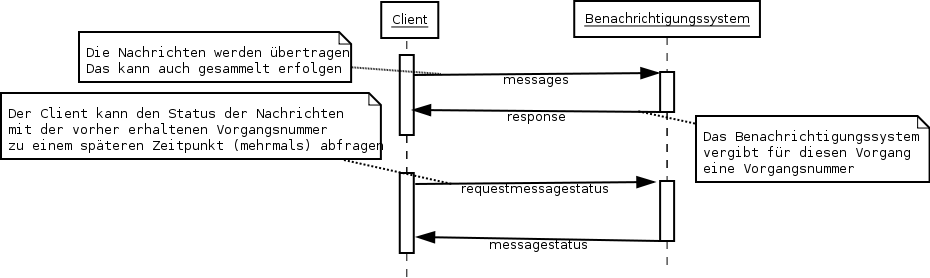
\includegraphics{xmlmessages.png}
	}
	\caption{XML Message Flow}
\end{figure}

\paragraph{Mögliche Nachrichten vom Client} Nachrichtenverwand, Statusabfrage
\paragraph{Antworten vom Server} Zuteilung von Nummern an Nachrichten, Statusantwort

Die Schnittstelle zu den externen Kommunikationsanbietern ist nicht Teil der Aufgabe und es wird vorrausgesetzt, dass diese von den externen Anbietern auch entsprechend abgesichert ist, um Missbrauch auszuschließen.

In den beiligenden XML Schema Dateien sind die Datentypen usw entsprechend genau spezifiziert, um hier schon vorher eine Validierung der Kommunikation vornehmen zu können.
Sollten die übertragenenen Daten nicht valid sein, erfolgt eine Fehlermeldung an den Client.

Dabei ist zu beachten, dass für die sichere Implementierung dieser Schnittstelle davon ausgegangen wird, dass sich der XML Parser korrekt verhält und keine Sicherheitslücken enthält.

\subsubsection{Beispiele für Nachrichten}
Siehe Abgabearchiv im Ordner \texttt{xml-samples}.

\section{Sicherheitsanalyse}

\begin{description}
	\item[Kompromittierung der Datenbank]
		Alle im System verwendeten Datenbanken sind sowohl auf DB- als auch auf OS-Ebene
		zu schützen. Ein Zugriff über die Applikationsebene ist authentifizierten
		Benutzern über eindeutig identifizierte Komponenten vorbehalten.
		
	\item[Kompromittierung des Betriebssystems]
		Alle eingesetzten Betriebssysteme müssen aktuell gehalten werden.
		
	\item[Mitschneiden von unverschlüsseltem Netzwerktraffic]
		Jede Kommunikation zwischen Modulen erfolgt verschlüsselt.
		
	\item[Social Engineering]
		Als Teil der organisatorischen Sicherheit muss das interne Personal entsprechend
		geschult werden um die Erfolgschancen von Social Engineering zu minimieren.

	\item[Manipulation von unverschlüsseltem Netzwerktraffic (Man in the Middle), Replay-Attacken]
		Jede Kommunikation zwischen Modulen erfolgt verschlüsselt und wird in beide
		Richtungen per 2-Way-SSL verifiziert.
		
	\item[Fehlende oder fehlerhafte Validierung der Eingabedaten]
		Alle Module validieren Eingabedaten und verweigern die Verarbeitung von
		formal oder semantisch ungültigen Daten.
		
	\item[Identitätsdiebstahl, Fehlerhafte Verteilung bzw. Verlust von Zugangsdaten]
		Diese Bedrohungen lassen sich einerseits durch organisatorische Maßnahmen beim
		Generieren und Verteilen der SSL-Zertifikate beim Einrichten der einzelnen
		Module aber auch durch Kundeninformation kontrollieren. Kunden müssen
		auf ihre Kreditkarte aufpassen.
		
	\item[(Distributed) Denial of Service]
		Die Kartenverwaltung ist als einziges inneres Modul ohne externe Schnittstellen
		relativ sicher vor DoS-Attacken. Bei allen anderen Modulen wird das Risiko
		minimiert, in dem Verbindungen ohne gültiges SSL-Zertifikat sehr schnell
		abgebrochen werden.
		
\end{description}

\end{document}


